\documentclass[../main.tex]{subfiles}

\begin{document}

\section{Results}

\subsection{Pilot}
We conducted a preliminary pilot version of the experiment to find reasonable variables to use for the final experiment. The pilot consisted of 10 participants who completed a version of the experiment with three seeds for each image and 21 $\alpha$-levels. With a Generalized Linear Model (GLM), we concluded that there was no effect of seed ($p=.38$). With a visual inspection on the effects of $\alpha$-values on agreement, we decided to remove $\alpha$-values that appeared redundant in showing the relation in order to have better measurements for the useful values.

\subsection{Participants}
After removing participants that did not satisfy the criteria listed above, our total number of participants was 542 ($M_{age}=31.17, \ SD_{age}=11.00, \ 234$ female) from 44 countries across the world. 


\subsection{Structural Models}
\begin{table}[!h]
	\centering
	\caption{Model Fit Indices}
	\begin{tabular*}{1\textwidth}{@{\extracolsep{\fill}} l c c c c c @{}}
		Model        & $\chi^{2}$ & \textit{df} & CFI & TLI & RMSEA \\ \hline
		CFA          & 33.92***   & 9           & .96 & .93 & .07   \\
		MIMIC 1      & 68.72***   & 29          & .94 & .91 & .05   \\
		MIMIC 2      & 68.00***   & 29          & .94 & .91 & .05   \\ \hline
		***$p<.001$. &
	\end{tabular*}
	\label{tab:fit}
\end{table}

\begin{figure}[!tb]
	\caption{Final MIMIC Model}
	\label{fig:finalmodel}
	\includegraphics[width=1\linewidth]{images/model3.pdf}
	{\textit{Note.} Rectangles are depicting observed variables while the oval is depicting the latent variable of interest. The numbers attached to each arrow represent the factor loadings. For the structural model, factors have been standardized on `Emotional'.\par
	*$p<.05$, **$p<.01$, ***$p<.001$}
\end{figure}


Our first model, the CFA on the shortened AEQ, resulted in a validation of the shortened questionnaire. The model fit can be seen in Table~\ref{tab:fit} under CFA. All fit indices, apart from the conservative $\chi^{2}$, were in the acceptable range (i.e., $>.90$ for CFI and TLI, and $<.08$ for RMSEA). All standardized factor loadings from the latent variable on the measured indices were significant ($p<.001$) and strong enough to justify interpretation ($>.80$). We interpret these results as evidence for our shortened version of the AEQ being adequate for measuring an individual's aesthetic experience.

For our first MIMIC model, we also obtained good fit measures, as seen in Table~\ref{tab:fit} under MIMIC 1. This model included an effect of sex, age, and nationality on aesthetic experience, and an effect of sex, age, and nationality on the proportion of agreement with the GAN. While the measurement part of the model remained largely unchanged, the new structural part of the model only showed a significant effect of nationality on aesthetic experience ($\beta = 0.01, p<.05$). This finding may have consequences for the AEQ itself, as \textcite{wanzerExperiencingFlowViewing2020} had mentioned that their own sample only included US participants. On the other hand, we did not find an effect of age and sex on aesthetic experience, unlike \textcite{wanzerExperiencingFlowViewing2020}. The most important finding here is that there was no effect of the latent aesthetic experience on the behavioral outcome variable of aesthetic judgement, which has important implications for the rest of our study.

For our second MIMIC model, illustrated in Figure~\ref{fig:finalmodel}, we made changes on theoretical bases. The fit indices were equally good, as seen in Table~\ref{tab:fit} under MIMIC 2, but we believe this second model makes more sense from a theoretical point of view. The standardized factor loadings were again very similar. Again, the effects of age and sex on aesthetic experience and aesthetic judgement were not significant. Nationality still has a significant effect on aesthetic experience here, but not on the cultural indicator. There was also no significant effect of aesthetic experience on aesthetic judgement here.



We can interpret these results as there being no effect of a person's demographic characteristics and their aesthetic experience on the outcome of the behavioral image rating task. This implies that the simple image comparison we used in our experiment is not influenced by seemingly relevant factors, pointing to a potential universal nature of aesthetic appreciation of the images we provided in the task. Furthermore, this will make our interpretations of the factors determining the aesthetic value of an image through GANalyze more generalizable.



\subsection{Behavioral Task}

\begin{figure}[!h]
	\caption{Behavioral Results from the Image Rating Task}
	\label{fig:psychometric_curves}
	\centering
	\begin{subfigure}{\textwidth}
		{\centering
			\includegraphics[width=.45\linewidth]{results/cont_asym.pdf}
			\hfill
			\includegraphics[width=.45\linewidth]{results/poly_regression.pdf}} \newline
		{\textit{Note.} (a)~Psychometric function for the proportion of chosen non-neutral images, illustrating that the estimated threshold value is approximately 0. Choosing the non-neutral image for a negative $\alpha$-trial corresponds with a disagreement with GANalyze and vice versa. Error bars were too small to display in the figure. \par (b)~Proportion of agreement with GANalyze with positive and negative $\alpha$'s taken together, fitted with quadratic regression.}
	\end{subfigure}
\end{figure}

To test the effect of different $\alpha$-values on image preference, we fitted a psychometric function on the data (Figure~\ref{fig:psychometric_curves}a). The figure shows that the relation between the $\alpha$-value used for image generation and the behavioral responses can be reasonably fitted with the typical psychometric function commonly found in psychophysical discrimination tasks. As expected, the estimated point of subjective equality (PSE) for the neutral and non-neutral image is at $\alpha = 0$ (99\% CI $[-0.00, 0.00]$). The estimated guess rate (equivalent to the lapse rate of negative $\alpha$'s) is 0.07 (99\% CI $[0.07, 0.08]$) and the estimated lapse rate is 0.17 (99\% CI [0.17, 0.18]).

\begin{table}[!h]
	\centering
	\caption{Polynomial Regressions}
	\begin{tabular*}{1\textwidth}{@{\extracolsep{\fill}} r c c c c r @{}}
		Predictor    & $b$      & \makecell{$b$\\$95\%$ CI} & $sr^2$ & \makecell{$sr^2$\\$95\%$ CI} & \makecell[c]{Fit}       \\ \hline
		(Intercept)  & 0.55**   & [0.50, 0.59]              &        &                              &                         \\
		$|\alpha|$   & 3.87**   & [3.05, 4.69]              & .39    & [.07, .72]                   &                         \\
		$|\alpha|^2$ & -10.03** & [-13.28, -6.78]           & .17    & [-.01, .34]                  &                         \\
		positive     & -0.05*   & [-0.09, -0.02]            & .03    & [-.02, .09]                  &                         \\
		             &          &                           &        &                              & $R^2 = .965$**          \\
		             &          &                           &        &                              & $95\%$ CI[$.85$, $.98$] \\
		             &          &                           &        &                              &                         \\
		(Intercept)  & 0.53**   & [0.48, 0.57]              &        &                              &                         \\
		$|\alpha|$   & 5.28**   & [3.46, 7.10]              & .12    & [-.01, .25]                  &                         \\
		$|\alpha|^2$ & -25.05*  & [-43.02, -7.08]           & .03    & [-.01, .07]                  &                         \\
		$|\alpha|^3$ & 39.63    & [-7.14, 86.41]            & .01    & [-.01, .03]                  &                         \\
		positive     & -0.05**  & [-0.09, -0.02]            & .03    & [-.01, .08]                  &                         \\
		             &          &                           &        &                              & $R^2 = .975$**          \\
		             &          &                           &        &                              & $95\%$ CI[$.87$, $.98$] \\ \hline
	\end{tabular*}
	\raggedright{\textit{Note.} A significant $b$-weight indicates the semi-partial correlation is also significant. \par
	$b$ represents unstandardized regression weights. \par
	$sr^2$ represents the semi-partial correlation squared. \par
	Square brackets are used to enclose the lower and upper limits of a confidence interval. \par
	*$p<.05$, **$p<.01$}
	\label{tab:reg}
\end{table}

We found a difference between the rating of high-$|\alpha|$ images for positive and negative $\alpha$-values (Figure~\ref{fig:psychometric_curves}b). People tend to agree more with GANalyze when it generates images that are supposed to be of lower aesthetic value compared to the neutral image. This difference is especially pronounced for the extreme variations. Table~\ref{tab:reg} shows the results of our polynomial regressions. A quadratic regression with the predictors $|\alpha|$, $|\alpha|^2$, and dummy variable \texttt{positive} explained 96.5\% of the observed variance. $|\alpha|$ and $|\alpha|^2$ both significantly predicted the proportion agreement with GANalyze. The \texttt{positive} variable was also significant, indicating an asymmetry in the appreciation of the generated high- and low-aesthetic images. We also fitted a cubic regression model, though the better fit could not be justified with the addition of another polynomial to the equation ($\Delta R^2=-.01, \  p=0.088$).

A two-way ANOVA with as factors the broad category labels and the position of the higher-$\alpha$ image revealed that there was no effect of broad category, $F(7,215)=0.009, \ p=1$, and no effect of stimulus position, $F(1,215)=0.000, \ p=.99$.


\subsection{GANalyze Parameters}
\begin{figure}[!h]
	\caption{Image Features}
	\label{fig:img_features}
	\includegraphics[width=1\linewidth]{images/results/img_features.pdf}
	{\textit{Note.} Figure depicting the change in average brightness, contrast, sharpness, and saturation from low-$\alpha$ to high-$\alpha$ images, illustrating that an increase in these features correlates with aesthetic preference. Values have been transformed from pixel intensities to z-scores for comparability.}
\end{figure}

The results from analyzing the image features of the 7,335 are displayed in Figure~\ref{fig:img_features}. Brightness, contrast, sharpness, and saturation all increase along with the $\alpha$-values. Notably, the curves for contrast and sharpness start slowing down at high positive $\alpha$-values. This asymmetrical shape was not expected and has theoretical implications.



The changes in color distribution for five random image sequences can be seen in Figure~\ref{fig:col_dists}. For the low $\alpha$-values, the colors tend to be clustered together on the lower end of the scale, indicating mostly dark gray colors. As the $\alpha$ increases, the color channels generally become wider and shift more to extreme values, either high or low. This means that the images are getting a larger diversity of colors that are also more intense.

\begin{figure}[!h]
	\caption{Color Distributions}
	\label{fig:col_dists}
	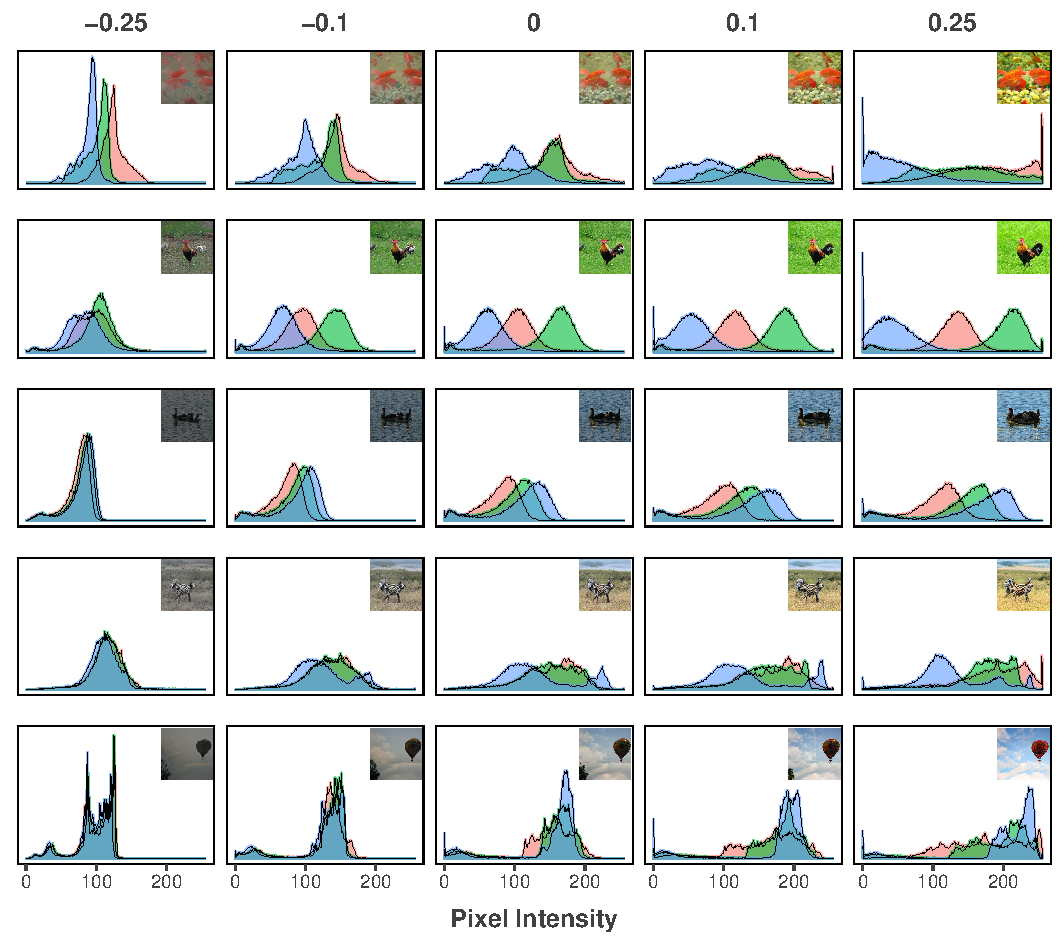
\includegraphics[width=1\linewidth]{images/results/col_dists_edit.pdf}
	{\textit{Note.} Figure depicting the distributions of RGB pixel intensities for five $\alpha$-values of five image sequences. The image corresponding to the distribution is embedded in the top-right of each histogram.}
\end{figure}






\end{document}